\chapter{Pozemkové úpravy}
\label{2-pu}

Tato kapitola se věnuje pozemkovým úpravám s~důrazem na~části, kterých se týka zásuvný modul vytvořený v~rámci této práce. Cílem není obsáhnout všechny informace o~pozemkových úpravách, to by stačilo na~samostatnou knihu a~takových již o~tomto tématu bylo publikováno nespočet, ale pouze čtenáři přiblížit nejdůležitější principy a myšlenky.

V~této kapitole bylo čerpáno ze zákona o pozemkových úpravách \citep{pu_zakon}, metodického návrhu \citep{metodicky_navrh}, skript \citep{pu_skripta} a dalších zdrojů \citep{pu_cr}.

\section{Pojem pozemkových úprav}
\label{pojem_pu}

Pozemkové úpravy zahrnují mnoho na~sebe navazujícíh činností, jejichž společným cílem je zlepšení podmínek pro~zemědelské hospodaření, zpřístupnění pozemků, zmírnění nepříznivých účinků vodní a~větrné eroze, zlepšení životního prostředí, zvýšení ekologické stability krajiny a~zachování či~obnova krajinného rázu. Děje se tak pomocí prostorového a~funkčního uspořádávání pozemků, pozemky se dělí a~scelují. K pozemkům se vyhotovují vlastnická práva a~s~tím související věcná břemena. Výsledky pozemkových úprav slouží jako podklady pro~obnovu katastrálního operátu.

Pozemkové úpravy jsou multidiscilinární obor, který využívá znalostí a~poznatků z~mnoha dalších oborů. Mezi ně patří zemědělství, krajinné a~územní plánování, geodézie, fotogrammetrie, vodohospodářství, ochrana životního prostředí, katastr nemovitostí a další.

\section{Význam pozemkových úprav}
\label{vyznam_pu}

Pozemkové úpravy mají význam jak pro~účastníky pozemkových úprav - vlastníky, stavebníky, obce - tak pro~obyvatele a~návštěvníky venkova, orgány státní správy, podnikatelské subjekty, správce inženýrských sítí a~zájmové organizace. Ve~výsledku mají tedy pozemkové úpravy dopad na~životy jednotlivců, společnosti a~celého státu.

Význam \zk{PU} pro vlastníky a~nájemce půdy:
	\begin{itemize}[leftmargin=1.5cm, noitemsep]
		\item přehledné a~jasné vlastnické vztahy
		\item vytyčené hranice pozemků v~terénu
		\item zajištěný přístup na~pozemky
		\item lepší tvar pozemků vhodných pro~racionální zemědělské hospodaření
		\item možnost uzavřít nájemní smlouvy na~přesné výměry a~hranice pozemků
		\item lepší organizace půdní držby
		\item zvýšená tržní cena pozemků
	\end{itemize}

Význam \zk{PU} pro zemědělské subjekty:
	\begin{itemize}[leftmargin=1.5cm, noitemsep]
		\item lepší tvar pozemků vhodných pro~racionální zemědělské hospodaření
		\item zajištěný přístup na~pozemky
		\item možnost uzavření nájemních smluv na~přesné výměry a~hranice pozemků
		\item možnost žádat o~dotace
	\end{itemize}

Význam \zk{PU} pro obce:
	\begin{itemize}[leftmargin=1.5cm, noitemsep]
		\item vyjasněné právnické vztahy v~území
		\item zpřístupnění a~zprůchodnění krajiny
		\item nalezení a~zapsání historického majetku obce
		\item podrobná dokumentace o~území
		\item realizace společných zařízení za~státní peníze
		\item podklad pro zpracování územního plánu
		\item zvýšená ekologická stabilita území
		\item protipovodňová ochrana obce
		\item podpora pěší turistiky a~cykloturistiky
		\item zkvalitnění života na~venkově
	\end{itemize}

Význam \zk{PU} pro orgány státní správy:
	\begin{itemize}[leftmargin=1.5cm, noitemsep]
		\item obnova katastrálního operátu
		\item odstranění zjednodušené evidence
		\item nová digitální katastrální mapa
		\item nové podrobné polohové bodové pole
		\item zvýšená retence krajiny
		\item snížení eroze
		\item zvýšená ekologická stabilita
		\item ochrana povrchových a~podzemních vod
	\end{itemize}

\section{Důvody pro pozemkové úprav}
\label{duvody_pu}

Důvodů k~zahájení pozemkových úprav býva obvykle několik, přičemž jeden či~více mají větší prioritu a~ostatní jsou spíše doplňující.

Nejčastější důvody pro~pozemkové úpravy:
	\begin{itemize}[leftmargin=1.5cm, noitemsep]
		\item území s~nedokončeným přídělovým nebo scelovacím řízením
		\item území s~množstvím jednoduchýh pozemkových úprav
		\item investiční záměr velkého rozsahu
		\item žádost vlastníků nadpoloviční výměry
		\item vyjasnění a~uspořádání vlastnických vztahů
		\item nevhodné tvary pozemků
		\item zpřístupnění pozemků a~krajiny
		\item nízká ekologická stabilita
		\item protipovodňová ochrana
		\item obnova katastrálního operátu
		\item návaznost na~sousední katastrální území
	\end{itemize}

\section{Cíle pozemkových úprav}
\label{cile_pu}

Cíle pozemkových úprav úzce souvisí s~důvody jejich zahájení. Snahou je soustředit se na~hlavní cíle a~zároveň neopomenout cíle vedlejší.

Hlavní cíle většiny pozemkových úprav:
	\begin{itemize}[leftmargin=1.5cm, noitemsep]
		\item vyjasnění a~uspořádání vlastnických práv
		\item zlepšení podmínek pro~racionální zemědělské hospodaření
		\item scelení roztříštěných pozemků jednoho vlastníka do~menšího počtu větších pozemků
		\item zlepšení tvaru pozemků pro~hospodaření
		\item zajištění přístupu na~pozemky
		\item zvýšení ekologické stability území
		\item zvýšení retence krajiny
		\item protipovodňová ochrana
		\item ochrana a~zúrodnění půdního fondu
	\end{itemize}

\section{Formy pozemkových úprav}
\label{formy_pu}

\subsection{Jednoduché pozemkové úpravy}
\label{jednoduche_pu}

Jak název napovídá, jednoduché pozemkové úpravy (\zk{JPU}) se týkají menší oblasti, obyčejně části katastrálního území.

Varianta \zk{JPU} bez~přechodu vlastnických práv se používala například po~roce 1990, kdy bylo potřeba narychlo umožnit hospodaření jednotlivým zemědělským subjektům, ovšem od~roku 2002 se již tyto \zk{JPU} neprovádějí.

V současné době se zahajují již jen \zk{JPU} se~zápisem vlastnických práv do~katastru nemovitostí. Tato varianta \zk{PU} se používá například v~pohraničních oblastech, kde jsou v~důsledku nedokončených přídělových řízení z~poválečného období nedořešené právnické vztahy, v~místech, kde vlastníci ve~velké většině souhlasí s~obnovou pozemků dle původní pozemkové evidence, nebo~v~oblastech, kde je nutné vyřešit specifický problém jako velké ohrožení pozemků půdní erozí, či~povodněmi.

\subsection{Komplexní pozemkové úpravy}
\label{komplexní_pu}

Komplexní pozemkové úpravy (\zk{KoPU}) zpravidla řeší nezastavěné území (extravilán) celého katastrálního území. Cílem \zk{KoPU} není pouze jeden konkrétní problém, jak~tomu může být u~\zk{JPU}, ale snaží se uspořádat pozemky v~širším kontextu. 

\section{Obvod a předmět pozemkových úprav}
\label{obvod_a_predmet_pu}

\subsection{Obvod pozemkových úprav}
\label{obvod_pu}

Obvodem pozemkových úprav se rozumí území dotčené pozemkovými úpravami, které je tvořeno jedním nebo více celky v~jednom katastrálním území. V~případě potřeby lze do \zk{ObPU} zahrnout i~navazující části sousedních katastrálních území. Hranice obvodu pozemkové úpravy býva obvykle rozdělena na vnitřní a vnější. Vnitřní hranice obvodu je nejčastěji určena hranicí mezi zastavěnou částí obce (intravilánem) a~nezastavěným územím (extravilánem). Vnější hranice zpravidla prochází~po hranici katastrálního území, po~hranici lesa, liniového objektu či~průmy\-slového areálu, může zasahovat i~do~sousedních katastrálních území. Při~volbě obvodu pozemkové úpravy by měly být zohledněny širší územní vztahy, neboť síť cest, ani~oblasti ohrožené erozí či~povodněmi se neřídí podle hranic katastrálních území. Z důvodu komplikovaného oceňování lesní pozemky zpravidla nebývají předmětem pozemkových úprav, obvod většinou končí na~jejich okraji.

\subsection{Předmět pozemkových úpravy}
\label{predmet_pu}

Všechny pozemky v~obvodu pozemkových úprav bez~ohledu na~dosavadní způsob využívání a~stávající vlastnické vztahy jsou předmětem \zk{PU}. Převážně se jedná o~zemědělské pozemky, ale~i~další pozemky v~extravilánu mohou být zahrnuty.

Pozemky v \zk{ObPU} se dělí na tyto kategorie:
	\begin{itemize}[leftmargin=1.5cm, noitemsep]
		\item \underline{pozemky v~\zk{ObPU} řešené} - pozemky, u~kte\-rých ve většině případů dochází ke~změnám v jejich poloze. Mohou být děleny, scelovány a~musí být zajištěna jejich přístupnost.
		\item \underline{pozemky v~\zk{ObPU} neřešené} - pozemky v~obvodu pozemkových úprav, u~kterých se pouze obnovují geodetické informace. U~těchto pozemků se zjistí průběh jejich hranic, označí se lomové body a~vypočítá se nová výměra ze~souřadnic v~S-JTSK. Do~\zk{PU} jsou zahrnuty proto, aby nová katastrální mapa neobsahovala vynechané části. Tyto pozemky se neoceňují.
		\item \underline{pozemky mimo \zk{ObPU}} - pozemky, které nejsou předmětem řízení o~pozemko\-vých úpravách. Nesměňují se, nezpřístupňují, nezaměřují a~ani neoceňují. Nerozhoduje o~nich pozemkový úřad.
	\end{itemize}

\section{Fáze pozemkových úprav}
\label{etapy_pu}

\subsection{Programová fáze}
\label{programova_faze}

Programová fáze je plně v kompetenci pozemkového úřadu. Pozemkový úřad shromažduje a~vyhodnocuje informace o~katastrálních územích, zjištuje zájem vlastníků, obcí a~nájemců o~provedení \zk{PU}. Na základě výsledného pořadníku katastrálních území a~finančních možností potom pozemkový úřad zahajuje pozemkové úpravy.

\subsection{Přípravná fáze}
\label{pripravna_faze}

Zahájení řízení o~pozemkových úpravavách je oznámeno veřejnou vyhláškou, kterou pozemkový úřad po~dobu patnásti dní vyvěsí na~úřední desku svou a~obcí, kterých se pozemkové úpravy budou týkat. Vlastníci jsou upozorněni na~nutnost trvale stabilizovat hranice pozemků. Pozemkový úřad s~jednoročním předstihem kontaktuje katastrální úřad, aby mohl zkontrolovat \zk{SPI}, \zk{SGI} a~opravit případné nesrovnalosti. Oba úřady, pozemkový a~katastrální, se dohodnou na~rozsahu pozemkové úpravy a~předběžně určí obvod. V~případě potřeby se pozemkový úřad spojí s~Výzkumným ústavem meliorací a~ochrany půdy (\zk{VUMOP}) a~zařídí aktualizaci \zk{BPEJ}. Dále také pozemkový úřad písemně informuje všechny dotčené orgány státní správy (\zk{DOSS}).

Ve~veřejném výběrovém řízení je vybrán zpracovatel, který začne shromaždovat podklady, zjišťovat stav území z~hlediska zemědělství, ochrany půdy, vody, vlastnických a~nájemních vztahů.

Po~zahájení \zk{PU} je svoláno úvodní jednání, na~které jsou pozváni všichni účastníci. Vlastníci jsou povinni prokázat vlastnická a~další věcná práva k pozemkům. Pozemkový úřad sdělí účastníkům důvody k~zahájení pozemkových úprav a~seznámí je s~účelem a~předpokládaným obvodem. Zpracovatel představí plánovaný harmonogram prací a~vysvětlí potřebu spolupráce s~vlastníky. Nutným úkolem úvodního jednání je také zvolit sbor zástupců. Ten musí být lichý, počet členů se pohybuje v~rozmezí od~pěti do~patnácti členů. Automatickými členy se stávají zástupce pozemkového úřadu a~zástupce obce. Sbor během \zk{PU} zastupuje vlastníky, spolupracuje se zpracovatelem, vyjadřuje se k~navrhovanému plánu společných zařízení a~ve~své činnosti pokračuje i~běhěm realizační etapy.

Při~zjišťování průběhu hranic se srovnává skutečnost se~stavem zakresleným v~katastrální mapě a~s~výsledky přechozích zeměměříčských prací. Lomové body vnitřní i~vnější hranice obvodu se v~terénu vyznačí a~později i~zaměří. Zjišťování se účastní zástupce obce, zpracovatel, zástupci pozemkového a~katastrálního úřadu a~zejména samotní vlastníci. Také se vytyčí a~označí vlastnické hranice pozemků, které nejsou v~terénu trvale stabilizovány.

Velmi důležitým krokem přípravné fáze je sestavení nároků vlastníků, na~jehož základě se posuzuje přiměřenost návrhu nového umístění pozemků. V~potaz se berou zejména výměry pozemků, vzdálenost těžistě pozemků od zvoleného referenčního bodu a~ocenění podle \zk{BPEJ}. Touto problematikou se podrobněji zabývá samostatná sekce (viz \ref{naroky}).

\subsection{Projekční fáze}
\label{projekcni_faze}

Po~přípravné fázi přichází na~řadu fáze projekční. Spočívá nejprve v~návrhu plánu společných zařízení, který byl dříve nazýván jako generel nebo~územní či~polyfunkční konstra.

Plán společných zařízení obsahuje čtyři základní části:
	\begin{itemize}[leftmargin=1.5cm, noitemsep]
		\item síť polních cest
		\item síť protierozních opatření
		\item síť vodohospodářských opatření opatření
		\item síť prvků systémové ekologické stability
	\end{itemize}

Po schválení plánu společných zařízení sborem zástupců a~zastupitelstvem obce se přikračuje k~samotnému vytvoření návrhu nového uspořádání vlastnických pozemků. Při~něm je nutné dodržet kritéria přiměřenosti výměr, cen i~dopravních vzdáleností pozemků jednotlivých vlastníků. V~průběhu pozemkových úprav, které mohou trvat i několik let, se vyhlašují takzvané kontrolní dny, kdy se schází sbor zástupců se~zpracovatelem, vyhotovují se předběžné návrhy nového uspořádání pozemků a~projednávají se s~účastníky \zk{PU}.

Když je návrh zpracovaný, vystaví se na~úřední desce obce a~pozemkového úřadu na~dobu třiceti dnů, během kterých mají vlastníci příležitost vznést své připomínky. Po~uplynutí této doby je svoláno závěrečné jednání, na~kterém se hodnotí výsledky pozemkových úprav a~hlasuje se o~schválení \zk{PU}. Pokud vlastníci minimálně tří čtvrtin výměry pozemků zahrnutých v~\zk{ObPU} souhlasí, je návrh pozemkových úprav schválen. To je podkladem pro~vydání prvního rozhodnutí o~schválení návrhu pozemkové úpravy. Rozhodnutí vydává pozemkový úřad, informuje o~tom veřejnou vyhláškou a~rozešle všem účastníkům část dokumentace, která se jich týká. Do patnácti dnů od~prvního rozhodnutí se vlastníci mohou odvolat, jakmile tato lhůta uběhne, nabývá první rozhodnutí pozemkového úřadu právní moci a~přistupuje se k~vydání druhého rozhodnutí pozemkového úřadu o~výměně nebo~přechodu vlastnických práv a~zřízení nebo~zrušení věcného břemene. Pozemkový úřad druhé rozhodnutí oznámí veřejnou vyhláškou, doručí jej katastrálnímu úřadu, vlastníkům a~dotčeným osobám. Proti druhému rozhodnutí se již není možné odvolat. Katastrální úřad obdrží dokumentaci o~novém geometrickém uspořádání pozemků a~jejich vlastnických práv.

\subsection{Realizační fáze}
\label{realizacni_faze}

Během realizační fáze se uskutečnuje schválený návrh \zk{PU}. Realizují se společná zařízení, vytyčuje se nové uspořádání pozemků a~lomové body hranic se označují trvalým způsobem. Dokončuje se nová digitální katastrální mapa (\zk{DKM}) a~soubor popisných informací. Katastrální pracoviště přijímá podklady pro~obnovu katastrálního operátu.

\subsection{Kontrolní fáze}
\label{kontrolni_faze}

Pozemkový úřad vyhodnocuje, zda bylo dosaženo vytyčených cílů. Kontroluje správ\-nost návrhu společných zařízení a~jeho funkčnost, přijímá zpětnou vazbu od~vlastníků, nájemníků, dotčených osob a~orgánů státní správy. Využívá těchto poznatků a~zkušeností při~dalších pozemkových úpravách.

\section{Sestavení vstupních soupisů nároků vlastníků}
\label{naroky}

Všichni vlastníci vstupují do~pozemkové úpravy se~svými pozemky, které mají určitou výměru, vzdálenost a~cenu. V průběhu pozemkové úpravy budou jejich pozemky scelovány do~větších výměr, budou narovávány jejich hranice a~budou přesouvány na nová místa. Na~konci pozemkové úpravy potom vlastníci dostanou nové pozemky, jejichž výměra, vzdálenost a~cena bude odpovídat pozemkům původním. Výsledkem je tedy to, že každý vlastník bude mít menší počet pozemků s~větší průměrnou výměrou, všechny budou mít vhodný tvar pro~zemědělskou činnost, budou přístupné a~budou chráněné proti erozi.

Soupisy vstupních nároků se vyhotovují pro všechny vlastníky pozemků, které alespoň částečně zasahují do~\zk{ObPU}, a~jsou závazným podkladem pro~návrh nového uspořádání pozemků.

Pro~sestavení soupisu nároků se používají tyto podklady:
	\begin{itemize}[leftmargin=1.5cm, noitemsep]
		\item katastrální operát - \zk{SPI} a~\zk{SGI}
		\item mapy dřívější pozemkové evidence
		\item výsledky podrobného zaměření hranice \zk{ObPU}
		\item údaje o~\zk{BPEJ}
		\item cenový předpis pro~oceňování pozemků
	\end{itemize}

Během zpracování \zk{PU} se odstraňují chyby v~katastrálním operátu, aby se v obvodu pozemkové úpravy nenacházel pozemek bez~vlastníka, a~také se kontrolují nabývací tituly, na~jejichž základě bylo vlastnictví zapsáno do~\zk{KN}.

Proces vyhotovení vstupních soupisů nároků je popsán v~následujících částech.

\subsection{Digitalizace mapových podkladů}
\label{digitalizace}

Pokud jsou mapové podklady v~grafické formě, je nutné je převést do~digitální podoby. V~územích, kde se provádí pozemkové úpravy, je nejčastěji k dispozici grafická katastrální mapa v~sáhovém měřítku 1:2880. Pro digitalizaci je nejprve nutné naskenovanou katastrální mapu pomocí identických bodů transformovat\ do~\zk{S-JTSK}. Do~\zk{S-JTSK} se kvůli identifikaci parcel vedených ve~zjednodušené evidenci natransformují i~mapy předchozích pozemkových evidencí. Mapy se poté digitalizací převedou do~vektorového formátu. Kód kvality podrobných bodů určených digitalizací je stanoven na základě měřítka katastrální mapy, viz tabulka \ref{tab:kody_kvality_digit}.

		\begin{table}[H]
		\begin{tabular}{|l|l|l|}
		\hline
		 kód kvality & měřítko katastrální mapy & základní střední souřadnicová chyba \\
		\hline
		\hline
		 6 & 1:1000, 1:1250 & 0.21 m \\ \hline
		 7 & 1:2000, 1:2500 & 0.51 m \\ \hline
		 8 & 1:2880 a jiné & 1.00 m \\
		 \hline
		\end{tabular}
		 \centering
		  \caption[Kódy kvality podrobných bodů určených digitalizací]{Kódy kvality podrobných bodů určených digitalizací (zdroj \citep{zakon_357})}
		  \label{tab:kody_kvality_digit}
		\end{table}

Základní střední souřadnicová chyba je dána vztahem:

\begin{equation}
	m_{xy} = \sqrt{\frac{(m_{x}^{2}+{m_{y}^{2}})}{2}}
\end{equation}

kde
\begin{tabbing}
\hspace{2em} \= \hspace{5em} \= \kill
	\> $m_{x}$	\> je střední chyba určení souřadnice $x$ \\
	\> $m_{y}$	\> je střední chyba určení souřadnice $y$
\end{tabbing}

\subsection{Kontrola souladu SPI a SGI}
\label{soulad_spi_sgi}

Pro všechny parcely zahrnuté do~obvodu pozemkové úpravy se provádí kontrola souladu souboru popisných a~geodetických informací. Kontrolují se druhy pozemků, parcelní čísla a~nesoulady v geometrickém a polohovém určení pozemku. 

Dále se porovnávají výměry parcel evidovaných v \zk{SPI} s~výměrou vypočtenou z~\zk{SGI}. Mezní odchylka výměr se vypočte pomocí vzorce z~tabulky~\ref{tab:odchylky_vymer}, kde $P$ je větší z~porovnávaných výměr v~metrech čtverečních.

		\begin{table}[H]
		\begin{tabular}{|l|l|}
		\hline
		 \begin{tabular}{@{}l@{}} kód kvality nejméně přesně \\ určeného bodu na~hranici parcely \end{tabular} & mezní odchylka [m\textsuperscript{2}] \\
		\hline
		\hline
		 3 & \(\displaystyle 2 \) \\ \hline
		 4 & \(\displaystyle 0.4*\sqrt{P}+4 \) \\ \hline
		 5 & \(\displaystyle 1.2*\sqrt{P}+12 \) \\ \hline
		 6 & \(\displaystyle 0.3*\sqrt{P}+3 \) \\ \hline
		 7 & \(\displaystyle 0.8*\sqrt{P}+8 \) \\ \hline
		 8 & \(\displaystyle 2.0*\sqrt{P}+20 \) \\
		 \hline
		\end{tabular}
		 \centering
		  \caption[Mezní odchylky výměr]{Mezní odchylky výměr (zdroj \citep{zakon_357})}
		  \label{tab:odchylky_vymer}
		\end{table}

\subsection{Vlastnická mapa}
\label{vlastnicka_mapa}

Ze~zpracovaných vektorových dat se následně vytvoří tzv. vlastnická mapa, ve~které na~rozdíl od~platné katastrální mapy má každá parcela svého vlastníka.

Vlastnická mapa se potom vytiskne v~barevném provedení, kde jsou parcely pro~každý list vlastnictví znázorněny jinou barvou nebo~šrafou. Součástí vytištěné vlastnické mapy je i~legenda.

Během procesu pozemkové úpravy se vlastnická mapa vyhotovuje dvakrát. Nejprve na~začátku \zk{PU}, kdy slouží k~projednávání soupisu nároku. Této variantě vlastnické mapy se také říká mapa nároků. Podruhé je vytvořena takzvaná mapa návrhu, která obsahuje nový stav navržených pozemků a~používá se k~seznámení vlastníků s~umístěním a~tvarem nových pozemků. Ukázka vlastnické mapy se nachází na~obrázku~\ref{fig:vlastnicka_mapa}.

	\begin{figure}[H]
		\centering
		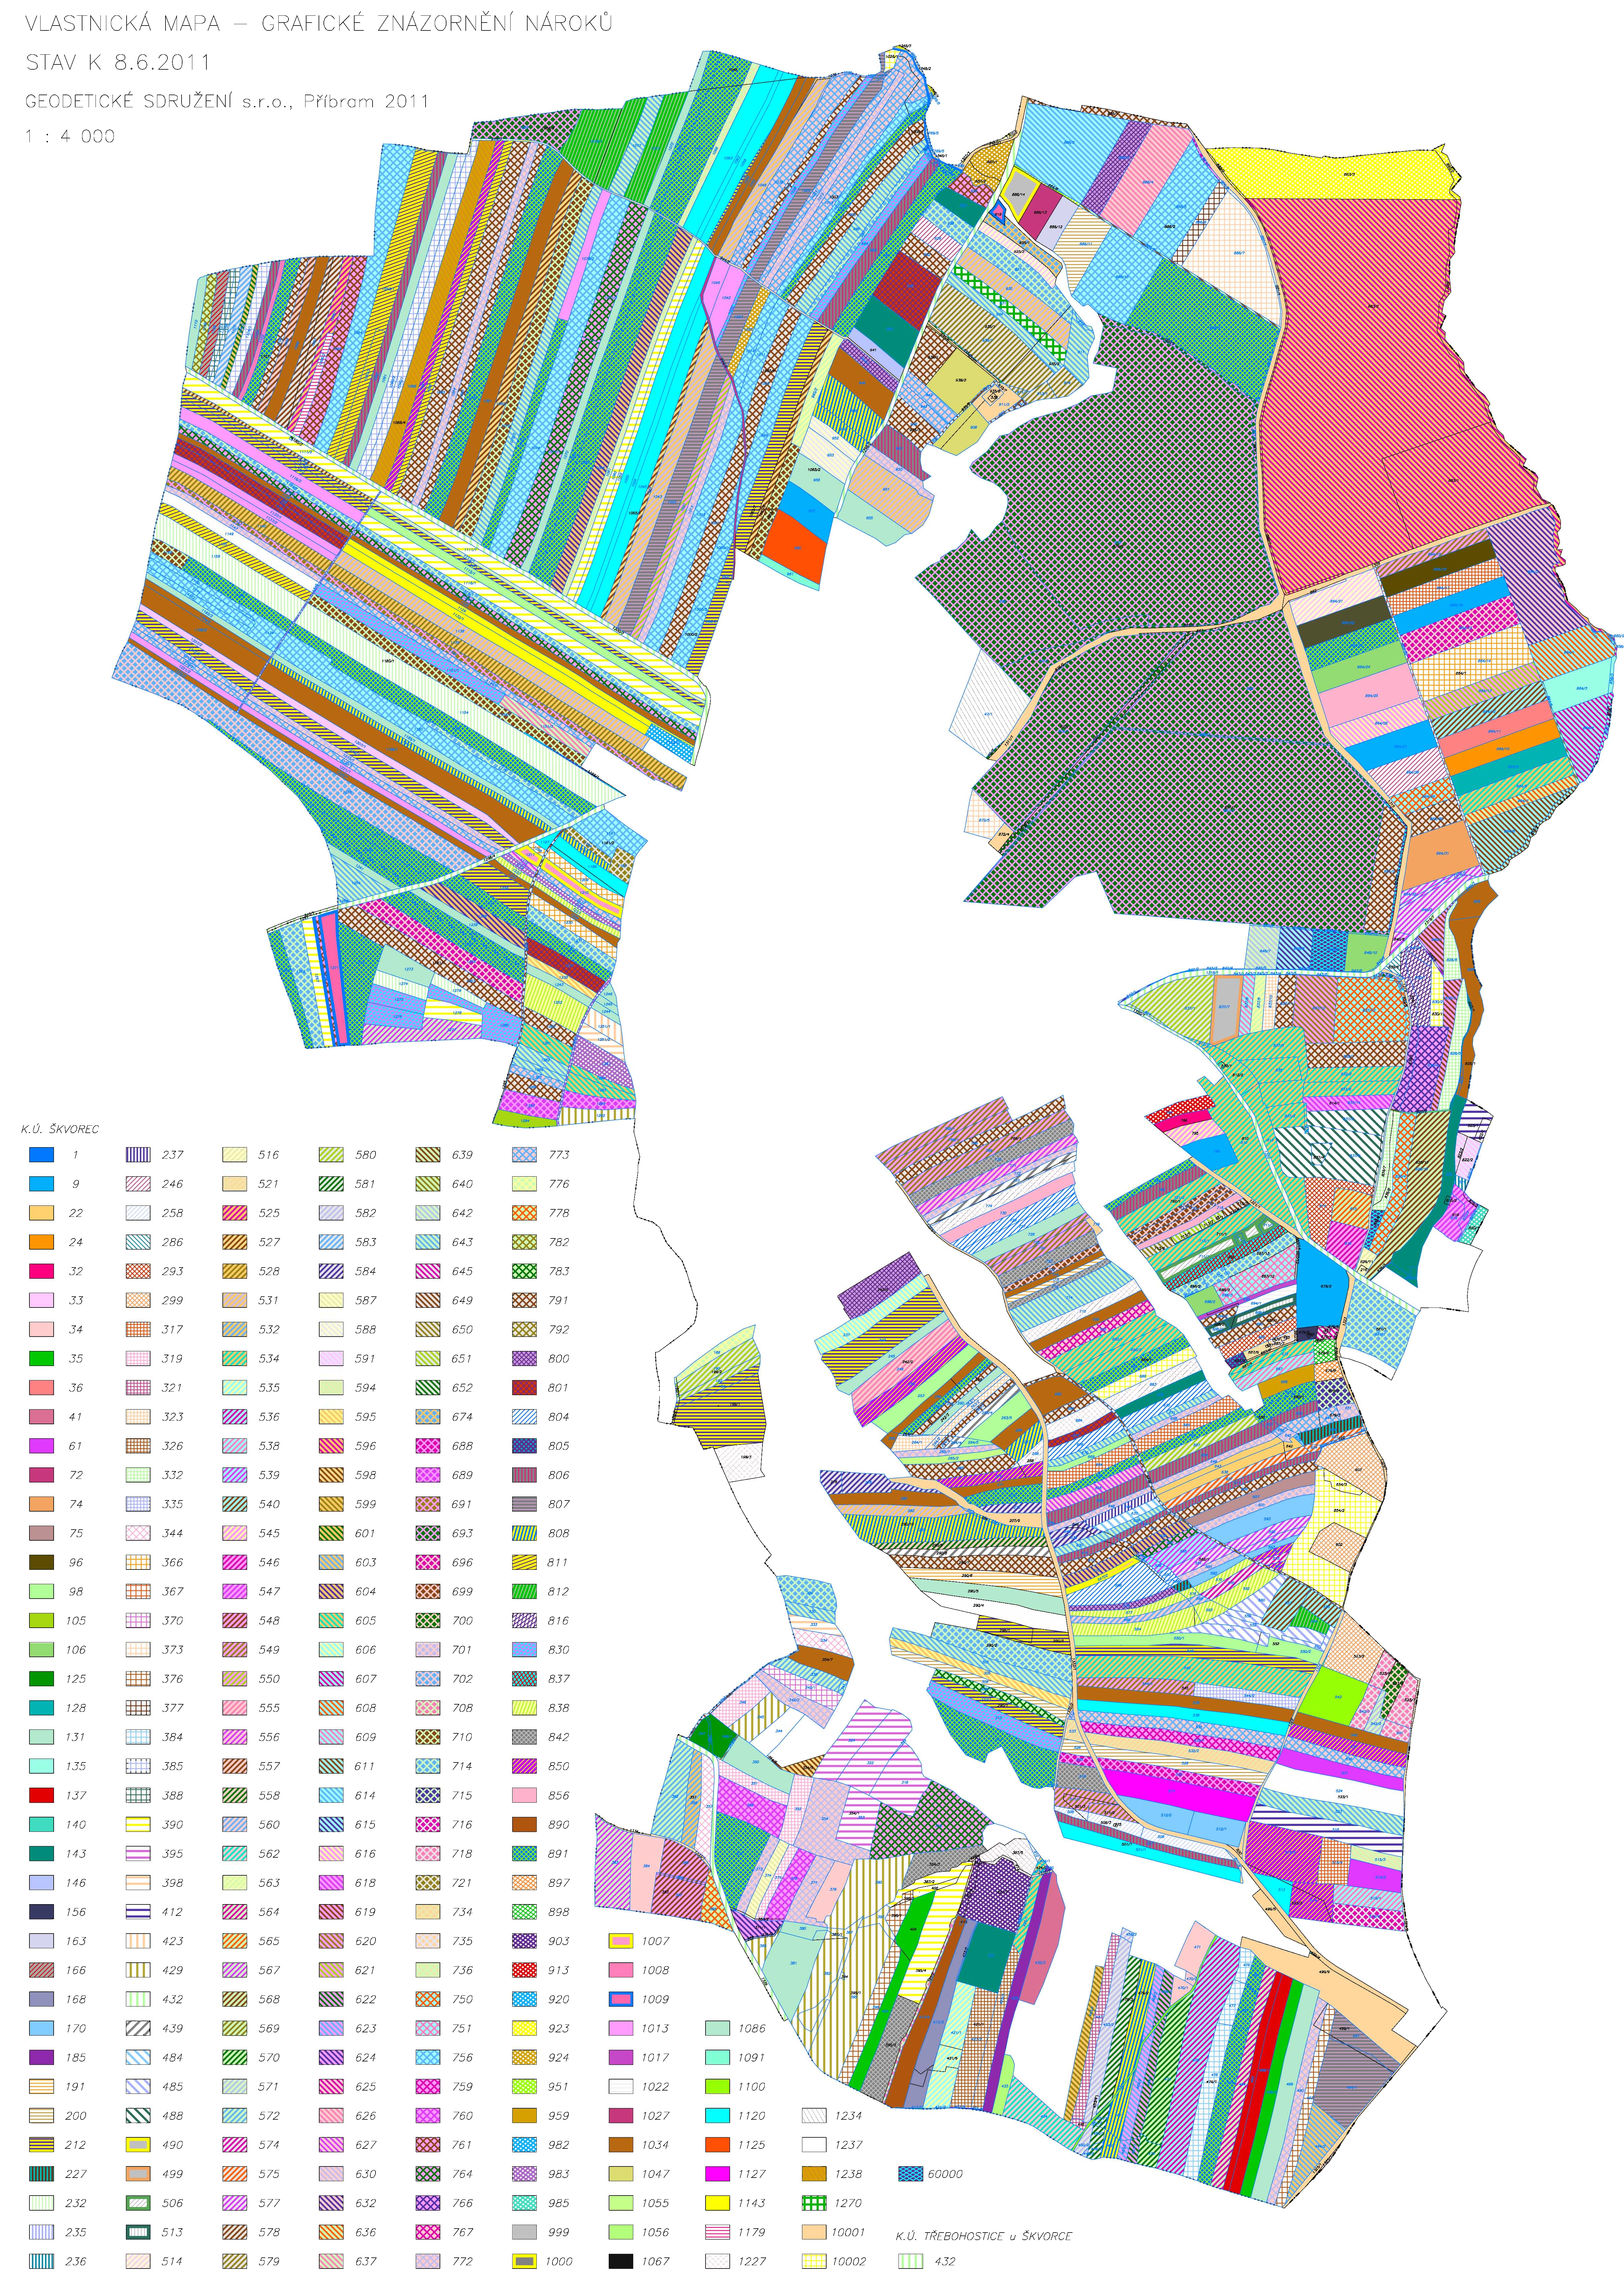
\includegraphics[width=.8\textwidth]{./pictures/vlastnicka_mapa.pdf}
		\caption[Vlastnická mapa]{Vlastnická mapa(zdroj:~\citep{skvorec})}
		\label{fig:vlastnicka_mapa}
 	\end{figure}

\subsection{Výpočet opravného koeficientu výměr}
\label{vypocet_ok}

Výpočtu opravného koeficientu výměr předchází zjišťování průběhu hranice obvodu pozemkové úpravy za~účasti vlastníků. Lomové body jsou v~terénu označeny, případně vytyčeny a~stabilizovány. Poté jsou tyto body s~požadovanou přesností (střední souřadnicová chyba $m_{xy}=0.14~m$, kód charakteristiky kvality bodu $3$) zaměřeny do systému \zk{S-JTSK} a provede se výpočet výměry obvodu pozemkových úprav ze~souřadnic. Součet výměr všech parcel v~obvodu pozemkové úpravy dá dohromady výměru obvodu pozemkových úprav podle katastru nemovitostí.

Opravný koeficient (\zk{OK}) se vypočte pomocí následujícího vztahu:

\begin{equation}
	OK = \frac{P\textsubscript{S-JTSK}}{P\textsubscript{KN}}
\end{equation}

kde
\begin{tabbing}
\hspace{2em} \= \hspace{5em} \= \kill
	\> $P_{S-JTSK}$	\> je výměra obvodu vypočtená ze souřadnic \\
	\> $P_{KN}$	\> je výměra obvodu určená součtem výměr parcel \\
	\> 				\> zahrnutých do obvodu podle katastru nemovitostí
\end{tabbing}

Výsledná hodnota opravného koeficientu je číslo, které by se mělo jen málo lišit od~$1$. Pokud je \zk{OK} menší než~$1$, pak se nároky zmenšují, v~opačném případě se nároky zvětšují. Opravný koeficient výměr slouží k~úpravě nároků podle skutečnosti.

\subsection{Ocenění pozemků}
\label{oceneni}

Všechny řešené pozemky se oceňují. K~oceňování se používají data s hranicemi \zk{BPEJ} od Výzkumného ústavu meliorací a půdy. Případnou změnu hranic \zk{BPEJ} podle~skutečného průběhu v~terénu musí odsouhlasit~\zk{VUMOP}. Ocenění se provede jako průnik vlastnické mapy a~hranic \zk{BPEJ}.

	\begin{figure}[H]
		\centering
		
\includegraphics[width=.5\textwidth]{./pictures/vumop.png}
		\caption[Logo Výzkumného ústavu meliorací a~půdy]{Logo Výzkumného ústavu meliorací a~půdy (zdroj:~\citep{vumop})}
		\label{fig:vumop}
 	\end{figure}

Nárokový list obsahuje nejen celkové ceny pozemků, ale také cenu za~metr čtvereční dle~kódu \zk{BPEJ} a~ceny částí pozemků dle~jednotlivých bonit.

Pozemky chmelnic, vinic, sadů, zahrad a~pozemků s~lesním porostem je povinné ocenit, v nárokovém listu se uvede cena pozemku uvede odděleně od~ceny porostu.

\subsection{Výpočet vzdálenosti pozemků}
\label{vypocet_vzdalnosti_pozemku}

Pro~všechny řešené pozemky je nutné vypočítat vzdálenost od~referenčního bodu. Vzdálenost pozemku se určí jako délka přímé spojnice těžiště pozemku a~referenčního bodu.

\subsection{Vlastní sestavení vstupních soupisů nároků vlastníků}
\label{vlastni_naroky}

Pro každého vlastníka (číslo listu vlastnictví) je sestaven soupis nároků neboli nárokový list, jehož hlavním výsledkem jsou tři hodnoty:
	\begin{itemize}[leftmargin=1.5cm, noitemsep]
		\item celková výměra pozemků - $P_{U}$
		\item celková cena pozemků - $C_{U}$
		\item průměrná vzdálenost pozemků - $D_{U}$
	\end{itemize}

\subsubsection{Prosté nároky}
\label{proste_naroky}

Nejprve je zapotřebí pro~každé \zk{LV} určit prosté nároky ve~výměře a~ceně. Vypočítají se jednoduchým součtem:

\begin{equation}
	P_{LV} = \sum\nolimits P_{p}
\end{equation}

kde
\begin{tabbing}
\hspace{2em} \= \hspace{5em} \= \kill
	\> $P_{LV}$	\> je prostý nárok ve výměře \\
	\> $P_{p}$	\> jsou výměry jednotlivých pozemků
\end{tabbing}

\begin{equation}
	C_{LV} = \sum\nolimits C_{p}
\end{equation}

kde
\begin{tabbing}
\hspace{2em} \= \hspace{5em} \= \kill
	\> $C_{LV}$	\> je prostý nárok v ceně \\
	\> $C_{p}$	\> jsou ceny jednotlivých pozemků
\end{tabbing}

\subsubsection{Průměrná vzdálenost pozemků}
\label{prumerna_vzdalenost_pozemku}

Průměrná vzdálenost pozemků pro~každé \zk{LV} se vypočte jako vážený průměr jednotlivých vzdáleností:

\begin{equation}
	D_{LV} = \frac{\sum\nolimits d_{p}*P_{p}}{\sum\nolimits P_{p}}
\end{equation}

kde
\begin{tabbing}
\hspace{2em} \= \hspace{5em} \= \kill
	\> $D_{LV}$	\> je průměrná vzdálenost pozemků \\
	\> $d_{p}$	\> jsou vzdálenosti jednotlivých pozemků \\
	\> $P_{p}$	\> jsou výměry jednotlivých pozemků
\end{tabbing}

\subsubsection{Upravené nároky}
\label{upravene_naroky}

Prosté nároky ve~výměře a~ceně se upravují opravným koeficientem, aby byly v~souladu se~skutečností. Průměrná vzdálenost se pomocí opravného koeficientu neupravuje.

\begin{equation}
	P_{U} = P_{LV}*OK
\end{equation}

kde
\begin{tabbing}
\hspace{2em} \= \hspace{5em} \= \kill
	\> $P_{U}$	\> je celková výměra pozemků \\
	\> $P_{LV}$	\> je prostý nárok ve výměře \\
	\> $OK$		\> je opravný koeficient
\end{tabbing}

\begin{equation}
	C_{U} = C_{LV}*OK
\end{equation}

kde
\begin{tabbing}
\hspace{2em} \= \hspace{5em} \= \kill
	\> $C_{U}$	\> je celková cena pozemků \\
	\> $C_{LV}$	\> je prostý nárok v ceně \\
	\> $OK$		\> je opravný koeficient
\end{tabbing}

\begin{equation}
	D_{U} = D_{LV}
\end{equation}

kde
\begin{tabbing}
\hspace{2em} \= \hspace{5em} \= \kill
	\> $D_{U}$	\> je průměrná vzdálenost pozemků \\
	\> $D_{LV}$	\> je průměrná vzdálenost pozemků
\end{tabbing}

Správnost sestavení soupisu nároků lze ověřit výpočtem sumy upravených nároků ve~výměře, která by se měla rovnat výměře obvodu \zk{PU} vypočtené ze~souřadnic:

\begin{equation}
	\sum\nolimits P_{U} = OK*\sum\nolimits P_{LV} = OK * \sum\nolimits \sum\nolimits P_{p} = OK*P_{KN} = \frac{P_{S-JTSK}}{P_{KN}} = P_{S-JTSK}
\end{equation}

kde
\begin{tabbing}
\hspace{2em} \= \hspace{5em} \= \kill
	\> $P_{U}$		\> je celková výměra pozemků \\
	\> $OK$			\> je opravný koeficient \\
	\> $P_{LV}$		\> je prostý nárok ve výměře \\
	\> $P_{p}$		\> jsou výměry jednotlivých pozemků \\
	\> $P_{S-JTSK}$	\> je výměra obvodu pozemkové úpravy vypočtená ze souřadnic \\
	\> $P_{KN}$		\> je výměra obvodu určená součtem výměr parcel \\
	\> 				\> zahrnutých do obvodu podle katastru nemovitostí	
\end{tabbing}

\subsubsection{Soupis nároků vlastníků}
\label{soupis_naroku_vlastniku}

V soupisu nároků vlastníků se pro~přehlednost a~jistotu, že se na~žádný pozemek nezapomnělo, uvádí i~pozemky mimo \zk{ObPU}. Neřešené pozemky se neoceňují, u~takových pozemků je v~nárokových listech zapsána pouze výměra podle \zk{KN} a~ze zaměření.

V soupisu nároků se uvádí:
	\begin{itemize}[leftmargin=1.5cm, noitemsep]
		\item číslo listu vlastnictví
		\item jména a~adresa vlastníka
		\item pozemky podle parcelních čísel v~obvodu i~mimo obvod \zk{PU}
		\item výměry pozemků
		\item druhy pozemků
		\item výměry částí pozemků dle \zk{BPEJ}
		\item celková výměra pozemků
		\item ceny pozemků
		\item ceny částí pozemků dle \zk{BPEJ}
		\item celková cena pozemků
		\item vzdálenosti pozemků
		\item průměrná vzdálenost pozemků
		\item opravný koeficient
		\item údaje o~omezení vlastnického práva
	\end{itemize}

Nárokové listy jsou po dobu patnácti dnů k dispozici k nahlédnutí na příslušném obecním úřadě a~jsou také rozeslány vlastníkům. Ti jsou vyzáni k~tomu, aby si zkontrolovali své nárokové listy a~vyjádřili souhlas podpisem.
 	
	\begin{figure}[H]
		\centering
		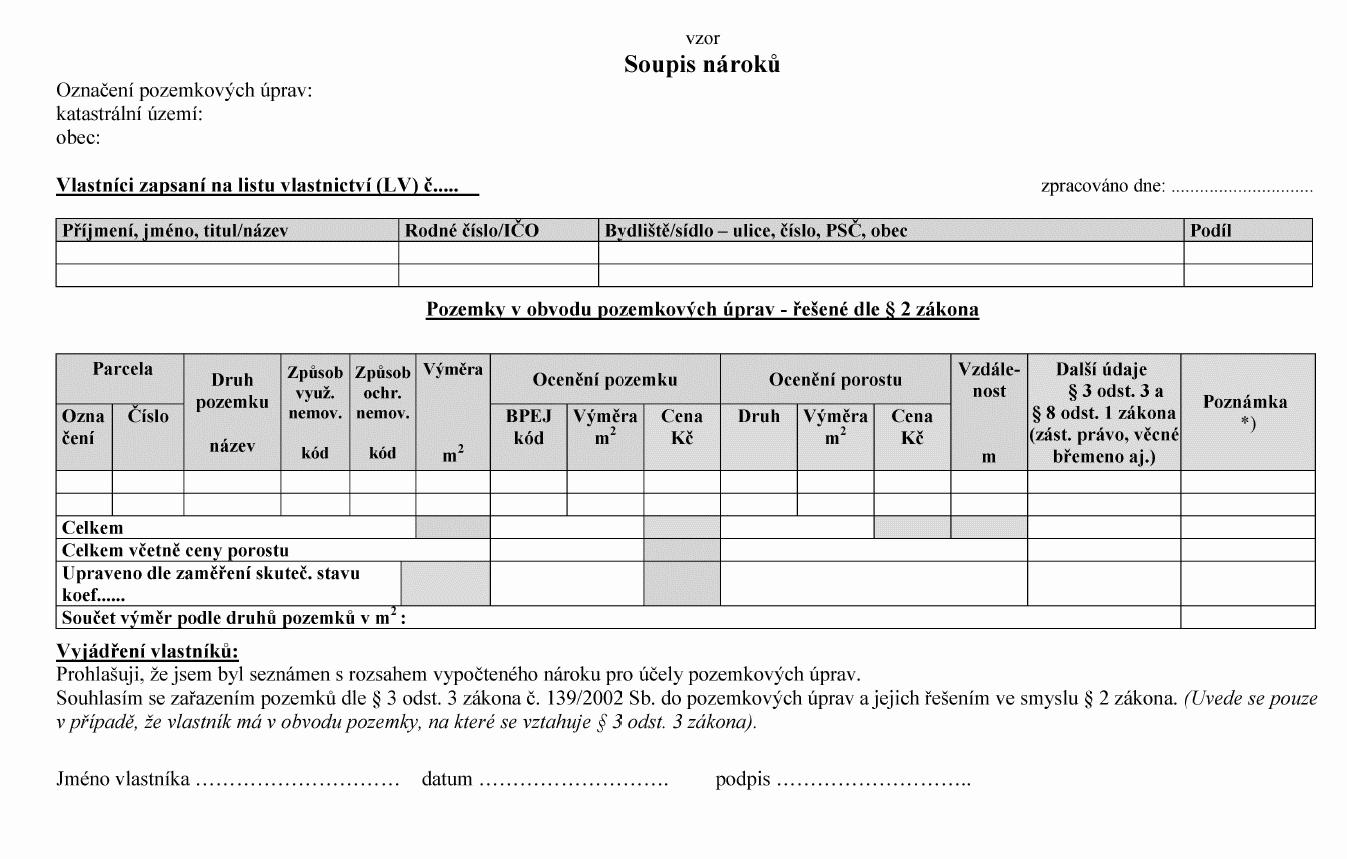
\includegraphics[width=.9\textwidth]{./pictures/soupis_naroku.png}
		\caption[Vzor soupisu nároků]{Vzor soupisu nároků (zdroj:~\citep{vyhlaska_13})}
		\label{fig:soupis_naroku}
 	\end{figure}

Vstupní soupisy nároků vlastníků patří mezi podklady pro~zpracování návrhu pozemkové úpravy. Celková výměra, cena a~průměrná vzdálenost nově navržených pozemků musí odpovídat pozemkům původním. Maximální rozdíly jsou dané zákonem o~pozemkových úpravách \citep{pu_zakon}.

\section{Programy pro zpracování pozemkových úprav}
\label{programy_pu}

Nezbytným nástrojem pro~zpracování pozemkových úprav je vhodný software, který podporuje práci s~navzájem propojenými geografickými daty a~databází. Tuto podmínku splňují všechny programy typu \zk{GIS} a~některé programy typu \zk{CAD}. Na~trhu je k dispozici několik programů, které se specializují čistě na~pozemkové úpravy, ale častěji se jedná o~extenze programů s~širším využitím. Tyto programy umožňují načítání vstupních dat ze~souboru \zk{VFK} a~podporují práci s~vektorovými i~rastrovými daty.

Všechny programy uvedené v~této sekci jsou distribuovány pouze pro~platformu Windows a~patří mezi~proprietární software.

\subsection{POZEM}
\label{pozem}

Systém POZEM je nadstavba programu Microstation nebo~jeho derivací určená pro~projektování komplexních pozemkových úprav. Nabízí zpracování všech etap \zk{KoPU}.

Funkčnost programu je možné rozdělit do~pěti skupin:
	\begin{enumerate}[leftmargin=1.5cm, noitemsep]
		\item \underline{Import dat} - import \zk{VFK} a dalších podkladů.
		\item \underline{Příprava dat} - výkresy je možné pomocí sady funkcí topologicky vyčistit a~připojit k~nim i~negrafické informace.
		\item \underline{Zpracování nároků} - na~základě mapových podkladů lze vypočítat výměru, cenu a~vzdálenost parcel. 
		\item \underline{Zpracování návrhu} - umožňuje návrh parcel s~okamžitým výpočtem výměry, ceny, vzdálenosti a~jeho porovnání s~nárokovými hodnotami.
		\item \underline{Výstupy} - export dat do~výměnného formátu pozemkových úprav (\zk{VFP}). Z~výsledného návrhu lze také zpracovat digitální katastrální mapu (\zk{DKM}) a~exportovat ji ve~formátu \zk{VFK}.
	\end{enumerate}

Výhody programu POZEM:
	\begin{itemize}[leftmargin=1.5cm, noitemsep]
		\item podpora zpracování všech etap \zk{KoPU}
		\item automatizace většiny procesů \zk{KoPU}
		\item vytváření sestav a~dokumentů podle platné legislativy
		\item export do~\zk{VFK} i~\zk{VFP}
		\item automatické aktualizace
	\end{itemize}

	\begin{figure}[H]
		\centering
		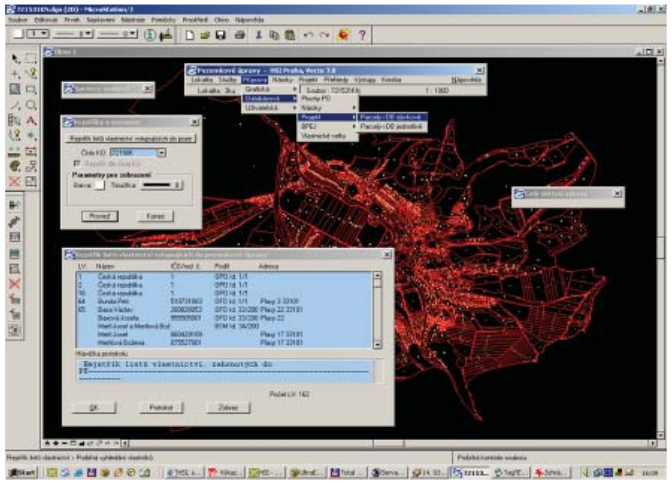
\includegraphics[width=.8\textwidth]{./pictures/pozem.png}
		\caption[Zpracování nároku v programu POZEM]{Zpracování nároku v programu POZEM(zdroj:~\cite{pozem})}
		\label{fig:pozem_obrazek}
 	\end{figure}


Všechny uvedené informace o programu POZEM vycházejí z oficiálních stránek produktu \citep{pozem} a~skript \citep{pu_skripta}.

\subsection{PROLAND}
\label{proland}

Dalším softwarových produktem pro~zpracování pozemkových úprav a~navazujících geodetických prací je program PROLAND. Jedná se o~rozšíření grafického systému KOKEŠ, které obsahuje sadu funkcí pro~automatické zpracování pozemkových úprav a~pro evidenci účastníků řízení.

Program PROLAND plně podporuje import a export dat ve výměnném formátu katastru nemovitostí.

Postup práce v programu PROLAND je podobný jako v~případě programu POZEM:
	\begin{enumerate}[leftmargin=1.5cm, noitemsep]
		\item \underline{Import dat} - načtení dat \zk{VFK} a dalších podkladů.
		\item \underline{Příprava dat} - možnost vyhotovení výkresů vektorizací rastrových souborů a~následná kontrola topologie.
		\item \underline{Zpracování nároků} - tvorba vstupních nároků včetně automatického přiřazení kodu BPEJ, přiřazení druhu a~způsobu využití pozemků odpovídající skutečnému stavu, ocenění parcel.
		\item \underline{Zpracování návrhu} - při~tvorbě nových pozemků se využívá především postupné dělení bloků půdy, které jsou vymezeny naprojektovanou kostrou území. V~konkrétních případech lze využít becných funkcí systému KOKEŠ. Program generuje soupisy nově navržených pozemků, přehled navržených parcel, souhrnou bilanci nároku a~návrhu.
		\item \underline{Výstupy} - export výstupů do~\zk{VFK} nebo~\zk{VFP}.
	\end{enumerate}

Výhody programu PROLAND:
	\begin{itemize}[leftmargin=1.5cm, noitemsep]
		\item možnost zpracování všech etap \zk{KoPU}
		\item automatizacké zpracování mnoha procesů \zk{KoPU}
		\item export dat do~\zk{VFK} i~\zk{VFP}
		\item pravidelné aktualizace
	\end{itemize}

	\begin{figure}[H]
		\centering
		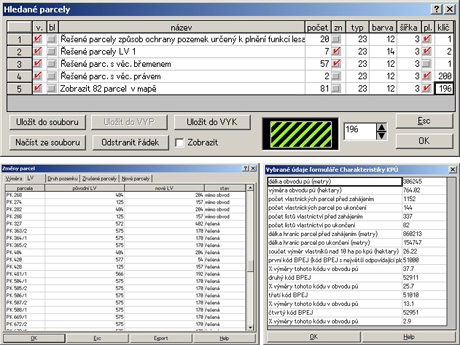
\includegraphics[width=.8\textwidth]{./pictures/proland.png}
		\caption[Komunikační výstupy z~programu PROLAND]{Komunikační výstupy z~programu PROLAND (zdroj:~\citep{proland_obrazek})}
		\label{fig:proland_obrazek}
 	\end{figure}

Veškeré výše uvedené informace týkající se programu POZEM vycházejí z~oficiálních stránek společnosti GEPRO~s.r.o. \citep{proland} a~skript \citep{pu_skripta}.

\subsection{TOPOL xT}
\label{topol_xt}

Na rozdíl od~obou předchozích programů typu \zk{CAD}, TOPOL~xT patří mezi geografické informační systémy. Nejširší oblastí využití programu TOPOL~xT je jednoznačně lesnictví, ale~své uplatnění najde i~při~zpracování pozemkových úprav. Poskytuje funkce pro~zpracování nároků, návrh nových parcel a~tvorbu všech nutných výstupů. Mezi výhody patří možnost tvorby vlastních uživatelských aplikací.

	\begin{figure}[H]
		\centering
		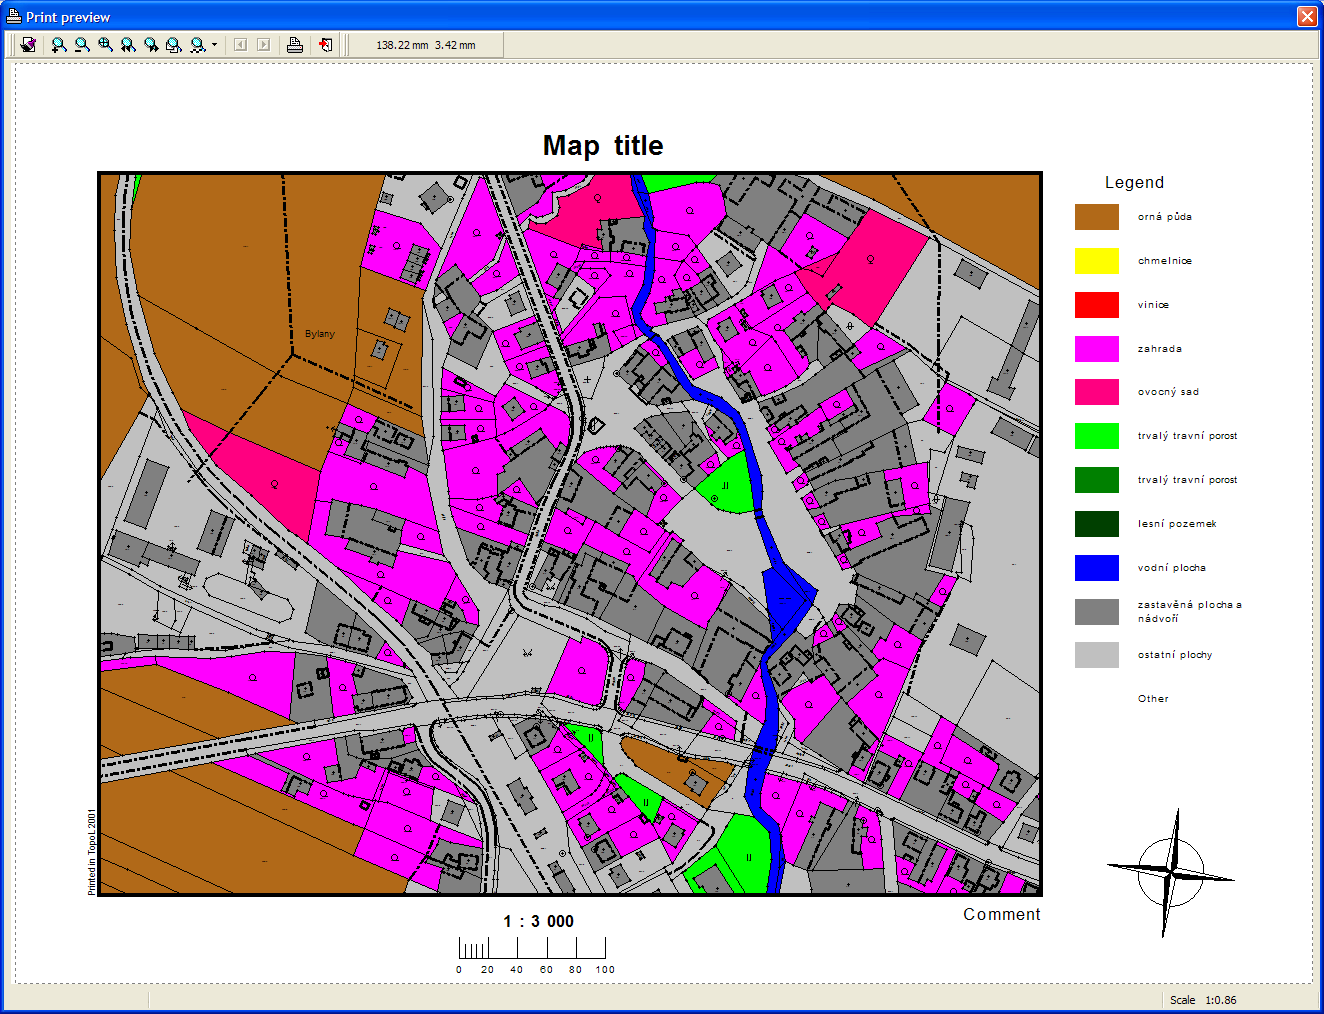
\includegraphics[width=.8\textwidth]{./pictures/topol.png}
		\caption[Náhled tisku v programu TOPOL xT]{Náhled tisku v programu TOPOL (zdroj:~\citep{topol})}
		\label{fig:topol_obrazek}
 	\end{figure}

Všechny informace týkající o~programu TOPOL~xT byly čerpány z~oficiálních stránek \citep{topol} a~skript \citep{pu_skripta}.